\documentclass[12pt,a4paper,oneside]{report}
\usepackage[utf8]{inputenc}
\usepackage[english]{babel}
\usepackage{amsmath}
\usepackage{amsfonts}
\usepackage{amssymb}
\usepackage{graphicx}
\usepackage[left=2cm,right=2cm,top=2cm,bottom=2cm]{geometry}
\author{Daniel Aguiar da Silva Carvalho}
\begin{document}
\sffamily
\begin{center}
\textbf{\large{Thesis Advancement Report 2014-2015 (First Year)}}
\end{center}

\begin{flushleft}
\textbf{Thesis title:} Trusted-SLA Guided on Multi-cloud Environments \\
\textbf{PhD. student:} Daniel Aguiar da Silva Carvalho \\
\textbf{Supervisor:} Chirine Ghedira-Guegan \\ 
\textbf{Co-supervisors:} Nadia Benani and Genoveva Vargas-Solar
\end{flushleft}

\begin{flushleft}
\textbf{Context}\\
\end{flushleft}

The data integration is a well-known and widely discussed problem in the database area. 
It consists in merging data from different data sources and granting a unified view of the data\footnote{Maurizio Lenzerini. Data integration: A theoretical perspective. In Proceedings of the Twenty-first ACM SIGMOD-SIGACT-SIGART Symposium on Principles of Database Systems, PODS ’02, pages 233–246, NY, USA, 2002.}. 
The cloud computing opens new challenges to data integration. The possibility of an unlimited access to resources that arises with the cloud model changes the way to process data.
In this context, some data integration approaches have been proposed.
The most addressed issue in these approaches is privacy, among others such as data protection, integrity and confidentiality. 

Applications and customer requirements naturally becomes more stringent. 
At this point, one single cloud can be out of resources while delivering and providing all requirements. 
In order to avoid this, cloud providers began to share their computing resources. 
This cloud collaboration is mentioned in the literature as multi-cloud, inter-cloud, cloud of clouds, hybrid cloud or federated cloud.
The new configuration of the cloud add more challenges to data processing, considering the large amount and diversity of data, and quality and security aspects of the integration.

In the cloud model, a common way of defining requirements and obligations between the \textit{cloud provider} and \textit{cloud customer} is through service level agreement (SLA) contracts. 
SLAs have been widely adopted in the cloud context. 
The proposal contributions are divided in two groups: (i) approaches focus on the SLA negotiation phase; and (ii) approaches for monitoring and allocation of resources in order to detect and avoid SLA violations. Among them, we identified one approach regarding data integration in a grid environment guided by an SLA model\footnote{Tiezheng Nie, Guangqi Wang, Derong Shen,Meifang Li,and Ge Yu. SLA-based data integration on database grids. In Computer Software and Applications Conference, 2007.}.

%In this context, we have two roles - the \textit{cloud provider} and \textit{cloud customer} - which have different requirements and obligations. In this model, a common way of specifying these requirements and obligations is through service level agreement (SLA) contracts agreed between the parts. 

%Cloud computing is an emerging paradigm which provides on-demand computing resources in a pay-as-you-go model. In this context, we have two roles - the \textit{cloud provider} and \textit{cloud customer} - which have different requirements and obligations. In this model, a common way of specifying these requirements and obligations is through service level agreement (SLA) contracts agreed between the parts. Naturally, as applications and customer requirements becomes more stringent, one single cloud can be out of resources while delivering and providing all customer's desires. To avoid this, collaborations between clouds (muli-cloud) in order to share resources takes place. 

%The possibility of having unlimited access to resources in this multi-cloud environment opens new challenges for data processing. For instance, the data integration problem that consists in merging data from different sources and providing a unified view of the data could take advantages from this environment. 
%The emergence of new architectures like the cloud opens new challenges to data processing. The possibility of having unlimited access to cloud resources and the “pay as U go” model make it possible to change the hypothesis under which current technology and solutions address the processing of huge volumes of data. Instead of designing processes and algorithms taking into account the limits on resources availability, the cloud sets the focus on the economic cost implied of using resources and producing results by parallelizing the use of computing resources while delivering data under subscription oriented cost models. 

Based on the aforementioned, we are interested in proposing a data integration approach in a multi-cloud hybrid environment guided by user preferences and service level agreements exported by different clouds.
To the best of our knowledge, we have not identified any other proposal concerning the use of SLAs combined with a data integration approach on a multi-cloud context.
This new approach brings different challenges and open issues: (i) which quality measures associated to data (that the data consumers what to query) and to the multi-cloud context should be present in SLAs? 
(ii) Considering the nature of the multi-cloud environment, how can quality and security aspects be guaranteed in the integration process? (iii) During the sources integration (services), it is necessary to monitor the chain of SLAs associated to different delivery models (IaaS, PaaS, etc) in order to guarantee no SLA violation in the others cloud subscriptions; and (iv) it is necessary the design of new matching-retrieving algorithms in order to select the best service composition according to the user requirements and the SLAs.

%The context imposes hence to consider SLA and different data delivery models. Indeed, we believe that given the volume and the complexity of query evaluation that includes steps that imply greedy computations, it is important to combine and revisit well-known data integration solutions and adapt them to this context. This can be done according to quality of service requirements expressed by the consumers and Service Level Agreement (SLA) contracts exported by the cloud providers that host data collections and deliver resources for executing the associated management processes.

%This project intends to address data integration in a multi-cloud hybrid context guided by user preferences statements and SLA contracts exported by different cloud providers and by several QoS measures associated to data collections properties: trust, privacy, economic cost. 

%The objective is to propose data integration (lookup, aggregation, correlation) strategies adapted to the vision of the economic model of the cloud such as accepting partial results delivered on demand or under predefined subscription models that can affect the quality of the results; accepting specific data duplication that can respect user preferences but ensure data availability; accepting to launch a task that contributes to an integration on a first cloud whose SLA verifies a given requirement rather than a more powerful cloud but with less quality guarantees in the SLA.

%Let us show an example from the domain of energy management to illustrate our problem. So for instance, we assume we are interested in queries like: \textit{Give a list of energy providers that can provision 1000 KW-h, in the next 10 seconds, that are close to my city, with a cost of 0,50 Euro/KW-h and that are labeled as green?} The question is how can the user efficiently obtain results for her queries such that they meet her QoS requirements, they respect her subscribed contracts with the involved cloud provider(s) and such that they do not neglect services contracts? Particularly, for queries that call several services deployed on different clouds.

%In our work we consider an example from the domain of energy management. My directors are working on two national projects in this domain. So for instance, we assume we are interested in queries like: Give a list of energy providers that can provision 1000 KW-h, in the next 10 seconds, that are close to my city, with a cost of 0,50 Euro/KW-h and that are labeled as green? The question is how can the user efficiently obtain results for her queries such that they meet her QoS requirements, they respect her subscribed contracts with the involved cloud provider(s) and such that they do not neglect services contracts? Particularly, for queries that call several services deployed on different clouds. This work is part of an international collaboration with the DiMAP, Federal University of Rio Grande do Norte.

\begin{flushleft}
\textbf{Synthesis of the research activities 2014-2015}\\
\end{flushleft}
During the first year of PhD project, we have been working on the state of the art. The idea is to be aware of all types of publications close related to the thesis proposal. To reach this, we proceeded with a literature analysis using a systematic mapping methodology. 

Briefly, the methodology consists in retrieving papers from scientific databases using the same search string. These papers are filtered according to an inclusion and exclusion criteria that should be defined based on the research interests. The papers will be classified in different categories (called facets) and for each facet in a specific dimension. The facets and dimension are defined based on the authors’ knowledge and interests. Taking the final papers collection, the abstracts should be read in order to classify each paper into the dimensions for each facet. 
This methodology allowed us to identify trends and open issues regarding our research topic and proposing an approach that fills some gaps and proposes an original data integration solution according to current trends in the area.

%The final objective of this first work is to show the research trends of data integration as a result of the emergence of the cloud and the characteristics associated to Big Data that require resources in order to be processed. In other terms, this methodology allowed us to identify trends and open issues regarding our research topic and proposing an approach that fills some gaps and proposes an original data integration solution according to current trends in the area.

This work performed, we thus have written an article that was \textbf{submitted} and \textbf{accepted} to the 26th International Conference on Database and Expert Systems applications (DEXA 2015) in the beginning of March 2015. We retrieved 1832 papers. 114 papers were selected based on our inclusion and exclusion criteria. This final data collection builds the state of the art to the thesis and, in the next step, we will perform an in-depth analysis of theses papers in order to (i) analyze what have been made and (ii) propose my approach.  

%This work performed, we thus have written an article that was \textbf{submitted} and \textbf{accepted} to the 26th International Conference on Database and Expert Systems applications (DEXA 2015) in the beginning of March 2015. This work has been made in collaboration with the Informatics’ Lab in Grenoble (co-supervisor Genoveva Vargas-Solar) and LIRIS Lab at INSA (co-supervisor Nadia Benani). The table below presents our results. We retrieved 1832 papers. 114 papers were selected based on our inclusion and exclusion criteria. This final data collection builds the state of the art to the thesis and, in the next step, we will perform an in-depth analysis of theses papers in order to (i) analyze what have been made and (ii) propose my approach.  

%\begin{center}
%\begin{tabular}{|c|c|c|c|}
%\hline 
%Database & Amount & Included & Excluded \\ 
%\hline 
%IEEE & 658 & 56 & 602 \\ 
%\hline 
%ACM & 649 & 31 & 618 \\ 
%\hline 
%Science Direct & 106 & 6 & 100 \\ 
%\hline 
%CiteSeerX & 419 & 21 & 398 \\ 
%\hline 
%Total & 1832 & 114 & 1718 \\ 
%\hline 
%\end{tabular}\label{fig1} 
%\end{center}

\begin{flushleft}
\textbf{Perspectives for the next year 2015-2016}\\
\end{flushleft}
Based on the publications extracted from the mapping process methodology, we will proceed the analysis of the current state of the art in order to formalize our proposal. The analysis will be the basis to our model proposal. As a natural result, we will write a paper describing our approach and a survey. In parallel, we will carry on the first steps of implementation of the proposed approach.
%This will be a proof of concept that can be presented to partners in energy domain.
The table below describes our intended calendar. The following activities are:
\begin{figure}[!h]
\center
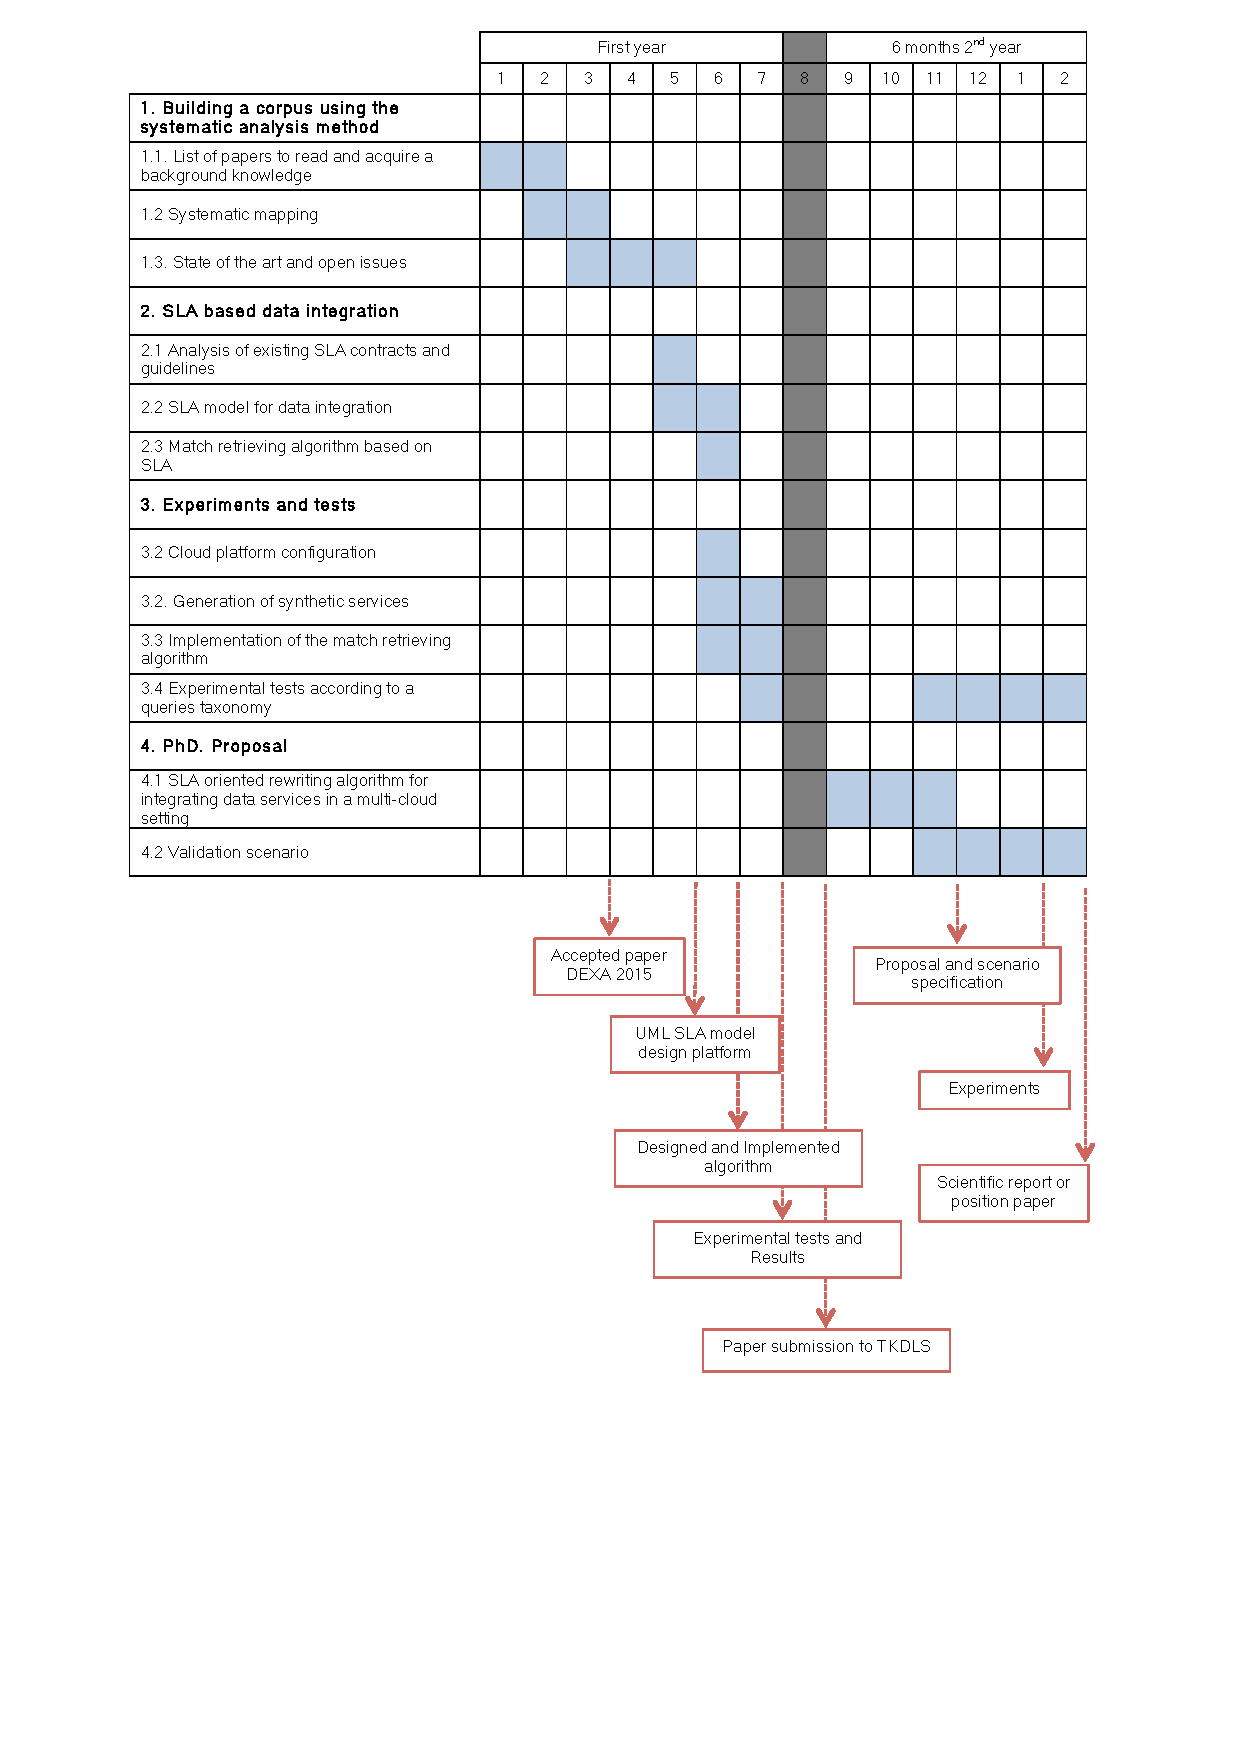
\includegraphics[scale=0.6]{calendario.pdf} 
\end{figure}
%\begin{enumerate}
%\item Paper submission: systematic mapping analysis.
%\item Analysis of the current state of the art.
%\item Identifying the list of SLA measures associated to data used by contracts.
%\item Proposal of SLA model(s) for data integration.
%\item Environment configuration and deployment of services using Open Stack.
%\item Description and implementation of match-retrieving algorithm.
%\item Evaluation and tests of our implementation. 
%\item Writing a report about the experiment.
%\item Approach proposal.
%\item Writing the paper that describes our approach and experiment results. 
%\item Writing the survey. 
%\end{enumerate}
%
%\begin{center}
%\begin{tabular}{|c|c|c|c|c|c|c|c|c|c|c|c|}
%\hline 
%- & Mar & Apr & May & June & July & Aug & Sept & Oct & Nov & Dec & Jan \\ 
%\hline 
%1 & • &   &   &   &   &   &   &   &   &   &  \\ 
%\hline 
%2 & • & • & • & • & • &   &   &   &   &   &  \\ 
%\hline 
%3 &   &   & • &   &   &   &   &   &   &   &  \\ 
%\hline 
%4 &   &   & • &   &   &   &   &   &   &   &  \\ 
%\hline 
%5 &   &   & • & • &   &   &   &   &   &   &  \\ 
%\hline 
%6 &   &   &   & • &   &   &   &   &   &   &  \\ 
%\hline 
%7 &   &   &   & • &   &   &   &   &   &   &  \\ 
%\hline 
%8 &   &   &   &   & • &   &   &   &   &   &  \\ 
%\hline 
%9 &   &   &   &   & • & • &   &   &   &   &  \\ 
%\hline 
%10&   &   &   &   & • & • & • &   &   &   &  \\ 
%\hline 
%11&   &   &   &   &   &   & • & • & • &   &  \\ 
%\hline 
%\end{tabular} 
%\end{center}






\end{document}